
\section{Introduction}

In this chapter, we will sample on BTCUSD and BTCUSDT dataset across all features and more specifically volume, side of the trade, speed of the market, and convergence of exchanges in various features. For simplicity reasons, when sampling takes place on all exchanges, the dataset will be aggregated to the 'second' or 'minute' interval (the 'minute' interval sampling will be used mostly for plotting purposes). In other occasions, the sampling will take place directly on raw tick data, nevertheless, in order to create the dataset for all exchanges, some sort of aggregation must be used, most probably in respect to time.

\subsection{Volume}

In this section, we will use volume along with different features of choice such as, positive-negative returns and buy-sell side. We will begin with buy-sell volume, while we illustrate how the sampling could end up in signal creation.

\subsubsection{Buy and Sell Volume}

The dataset is created by classifying the volume into buy and sell volume, depending on the side of the trade. This classification is taking place directly on tick data. Then, the dataset is aggregated (summation) on the 'second' time interval, where two columns are created: one for the buy volume and one for the sell volume. This procedure is used for all exchanges and as we have shown, all exchanges should be used (see \ref{fig:cum}). 

The latter results to a 10 column dataset where 5 columns are created for the buy volume and 5 columns for the sell volume (one column for each exchange). Lastly, the 5 columns of each side, are summed row-wise in order to create one column for buy and one column for sell volume. The last columns represent the volume that took place on all exchanges after being classified as buy and sell.

In order to model the two volumes, we will use a Hawkes process. To provide the reader with a brief explanation of the Hawkes process, we shall begin with a Poisson process, which models the number of occurences at certain time intervals. The key takeaways from Poisson processes are that the expected rate of these occurrences \( \lambda \) is stable (homogeneity) and that the expected rate of occurrences at a future time interval is independent of past occurrences. 

In order to study more complex phenomena, a Non-homogeneous Poisson process could be used, where the future events are still independent of past phenomena, but \( \lambda \) is now a function of time. This particular idea fits somewhat with market behavior, in that the expected rate of returns (or as we will later show), the expected rate of volume traded, does seemingly not behave independently of the time interval, but fluctuates locally. There are certain periods of time where the volume that is expected to be traded is higher (moments of behavior co-ordination). For the function \( \lambda(t) \) to be called a deterministic function (and also non-homogeneous Poisson process) there are certain axioms that need to be held. This function then is called an “Intensity function”.

Lastly, in addition to the above, if the intensity function is not stable, but is affected by the history of the timeseries up to time \(t\), the process is called Hawkes process. A Hawkes process is a self-exciting process, which its past events affect the current value of the process. There also exist other similar approaches to Hawkes, such as convolutional neural networks which are mostly used for image classification that use a weighted average of previous values. The problem with this approach, contrary to Hawkes is that this approach would enforce static dependencies while Hawkes intensity function uses the \(N(t)\) counting process as a positive reinforcement that decays exponentially in such a way that past events that are close to time \(t\), affect the value of the function much more than, say older events that are further away from \(t\). 

In a volume specific example the formula would be:
\[ \lambda(t|H_t) = \lambda_0(0|H_0) + \sum_{i=1}^{N(t)}\text{Vol}(i) \cdot e^{-\delta(t-T_i)} \]
where \(\lambda_0(0|H_0) \) is the initial intensity and \( \delta \) would be a positive dampening coefficient that implies the rate at which the function decays.

Using a Hawkes process with \( \delta = 0.2 \) and \( \lambda_0 = 0 \), we modeled the buy and sell volume, and upon the new dataset, we sampled using two parallel moving averages, one slow (larger scope) and one faster (smaller window). The sampling took place, when the fast MA exceeded the slow MA by a threshold. This way, we can have an overview of the buy and sell volume surges. First thing to notice, is that most of the points sampled from the two volumes are different (see \ref{fig:hawkes1}). There is an oversampling in sudden price action and no sampling at all when price goes sideways. Furthermore, the buy volume, is found mostly in local maxima and the sell volume in local minima, which is to be expected.

\begin{figure}[H]
    \centering
    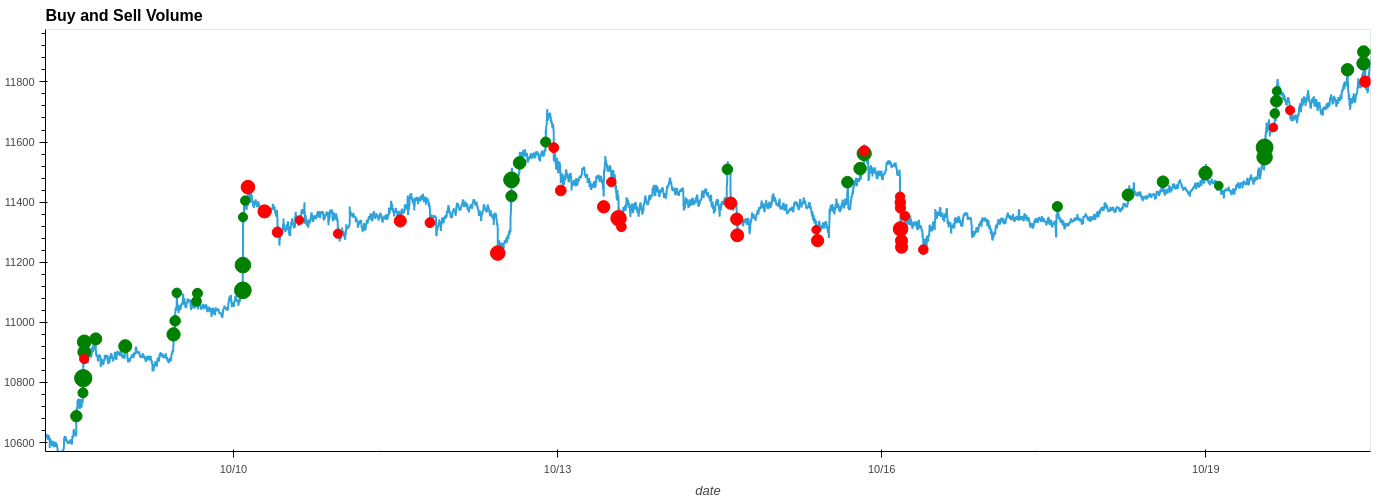
\includegraphics[width=10cm, height = 4cm]{hawkes1.png}
    \caption{An example of buy (green circle) and sell (red circle) volume. The size of the markers, correspond to the amount volume traded.}
    \label{fig:hawkes1}
\end{figure}


At this point, we decided to disregard the mandatory positive counting process and instead use a process that could take negative values. That process would be the difference between positive and negative volumes and it would no longer be a Hawkes process. The first results of our experimentation showed that when the buying side was far greater than the negative selling side, the process would be excited by a positive value and vice versa. Thus, this process could also take negative values, but even if a large negative selling volume appeared, it would take a couple of steps for the function to actually get affected enough and fall below zero (lagging). We consider it natural for sellers to affect buyers and vice versa, and we decided to follow this idea because simple volume self-excitation was not enough.

We used the following custom intensity function: 
\[ \lambda(t|H_t) = \lambda_0(0|H_0) + \sum_{i=1}^{N(t)}(\text{Vol}_{\text{Buy}}(i) - \text{Vol}_{\text{Sell}}(i)) \cdot e^{-\delta(t-T_i)} \]

After modelling the above difference, we used two moving averages, one slow (larger scope) and one faster (smaller window), as above. We then decided to sample based on two different factors, thus creating 4 states. The rationale behind the 4 states, is that we could sample not only when the volume difference spikes, but also when the spike ends, signaling the end of the price action.
The two factors are:
\begin{itemize}
\item Faster MA over slow MA and vice versa (setting a threshold as above)
\item Sign of the difference 
\end{itemize}

And the four states:
\begin{enumerate}
\item Fast moving average of our process would exceed the slow-moving average, indicating there is incoming positive volume (immediate past) at greater rate than the slow-moving average (larger past time window) and the Buyers volume exceeds the Sellers volume.
\item Fast moving average of our process would exceed the slow-moving average, indicating there is incoming positive volume (immediate past) at greater rate than the slow-moving average (larger past time window) and the sellers volume exceed the Buyers volume. We believe this to be a significant indicator for sampling (specifically a shorting the market indicator) because it shows that although there has been a large Buyers rate recently, Sellers appear to significantly take over the reins. Additionaly, it could also indicate the end of an upward price move.
\item Fast moving average of our process would fall below the slow-moving average, indicating there is incoming negative volume (immediate past) at greater rate than the slow-moving average (larger past time window) and the Sellers volume exceeds the Buyers volume.
\item Fast moving average of our process would fall below the slow-moving average, indicating there is incoming negative volume (immediate past) at greater rate than the slow-moving average (larger past time window) but the Buyers volume would exceed the Sellers volume. We also believe this to be a significant indicator for sampling (specifically a longing the market indicator) because it shows that although there has been a large Sellers rate recently, Buyers appear to significantly take over the reins. Additionaly, it could also indicate the end of an downward price move.
\end{enumerate}

In the figure \ref{fig:hawkes2}, we can see an example of the states. Upon carefull inspection of the local minima, we observe increased sell volume (upper graph, red triangle), with the fast MA above the slow one (lower graph, green circle). In many of these occasions, a reversion occurs right away. The latter is a state 2 example. Using the same notion, we distinguish a state 4 example, by observing that at local maxima, the increased buy volume (upper graph, green triangle) is accompanied with the fast MA being under the slow one (lower graph, red cross). In many occasions, a reversion in the price occurs. 

\begin{figure}[H]
	\centering
    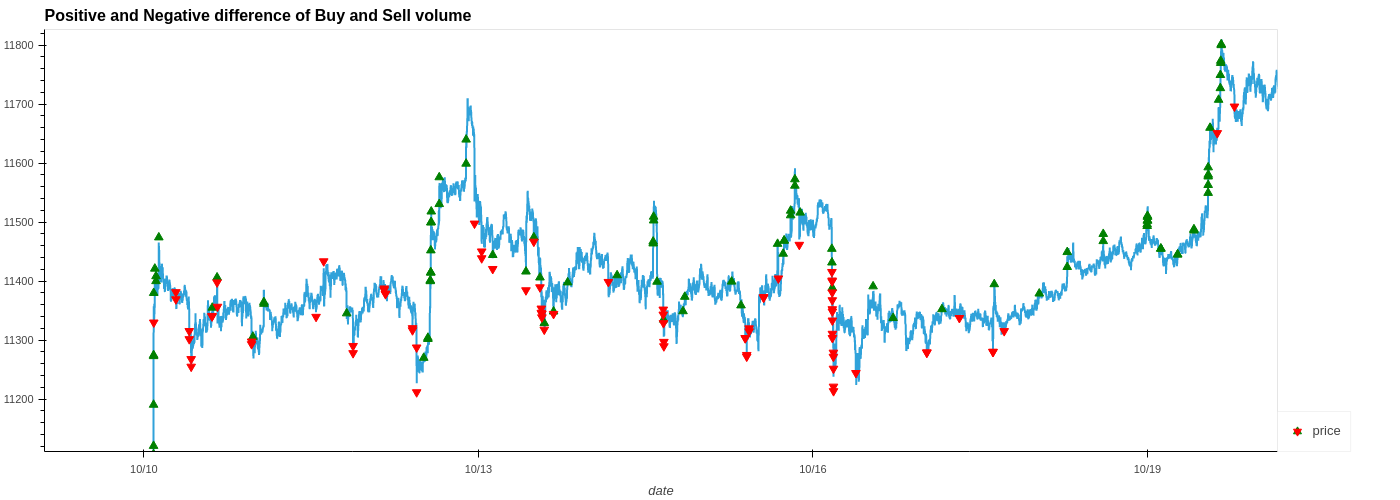
\includegraphics[width=12cm, height = 4cm]{hawkes2.png} \\
    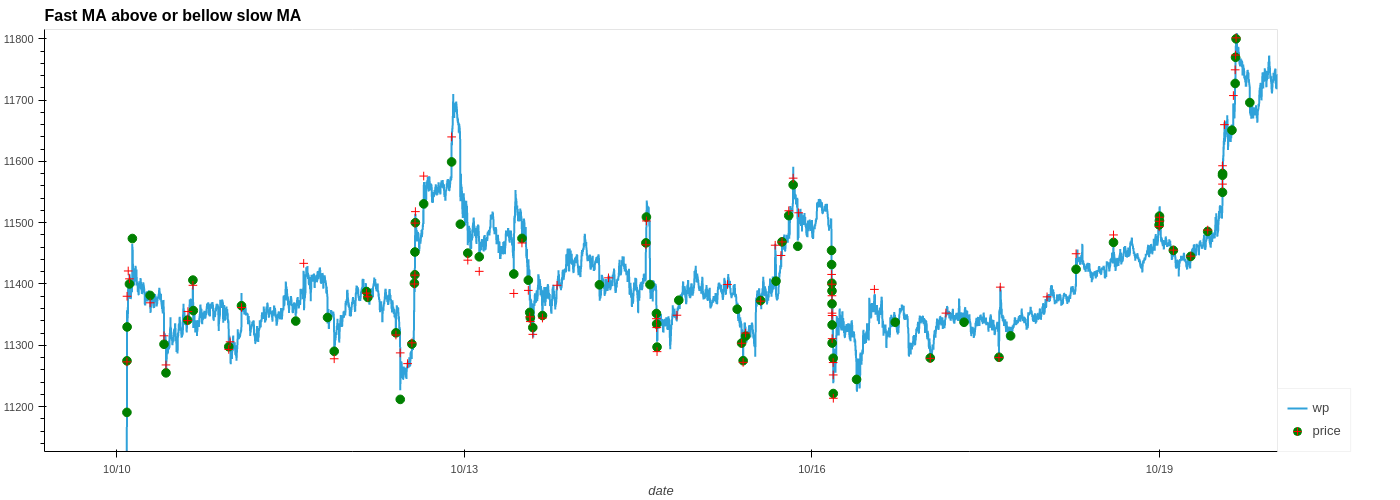
\includegraphics[width=12cm, height = 4cm]{hawkes3.png} \\
	\caption{An illustration of the four states. The first graph corresponds to the first factor and the second graph to the second factor. In the first graph, the green arrows indicate buy volume and the red ones, sell volume. In the second graph, the green circle corresponds to Fast MA > Slow MA, while the red cross, corresponds to the exact opposite.}
    \label{fig:hawkes2}
\end{figure}


The reader should keep in mind, that the sampling took place in the 'second' timeframe, while the price in the figure above, is plotted from the 'minute' timeframe, using the mean price during that minute. Therefore, the real volatility cannot be grasped by this graph, and some points seem to wander off the price plot. In order to bypass that shortcoming, and furthermore, to illustrate visually how modelling - sampling - parameters look like, a zoom-in figure, with price displayed in seconds will be presented.


\begin{figure}[H]
	\centering
    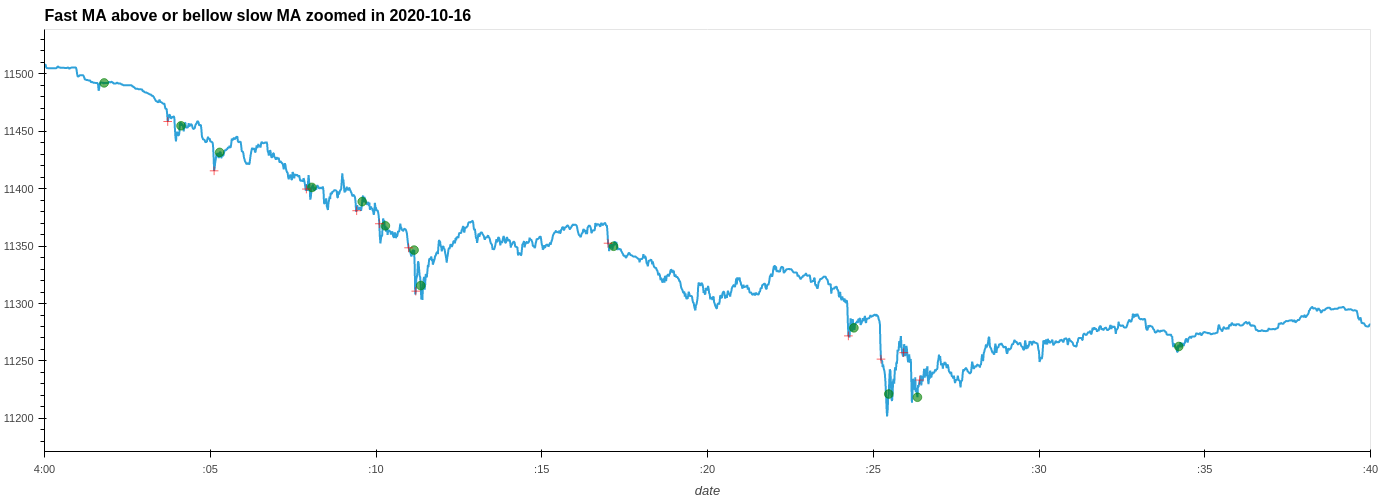
\includegraphics[width=12cm, height = 4cm]{hawkeszoom1.png} \\
    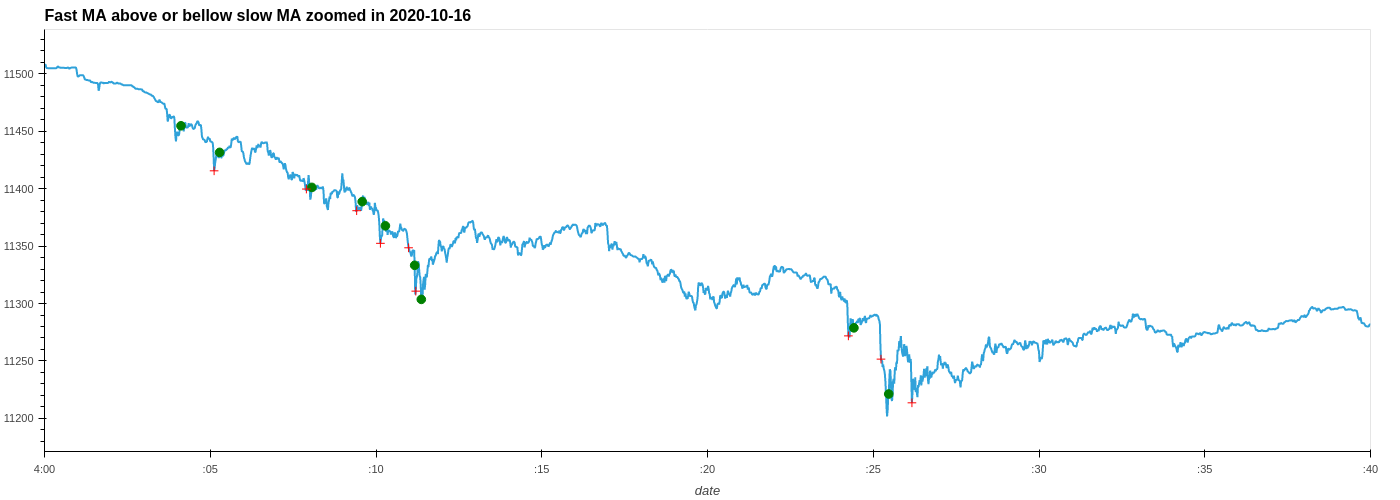
\includegraphics[width=12cm, height = 4cm]{hawkeszoom2.png} \\
    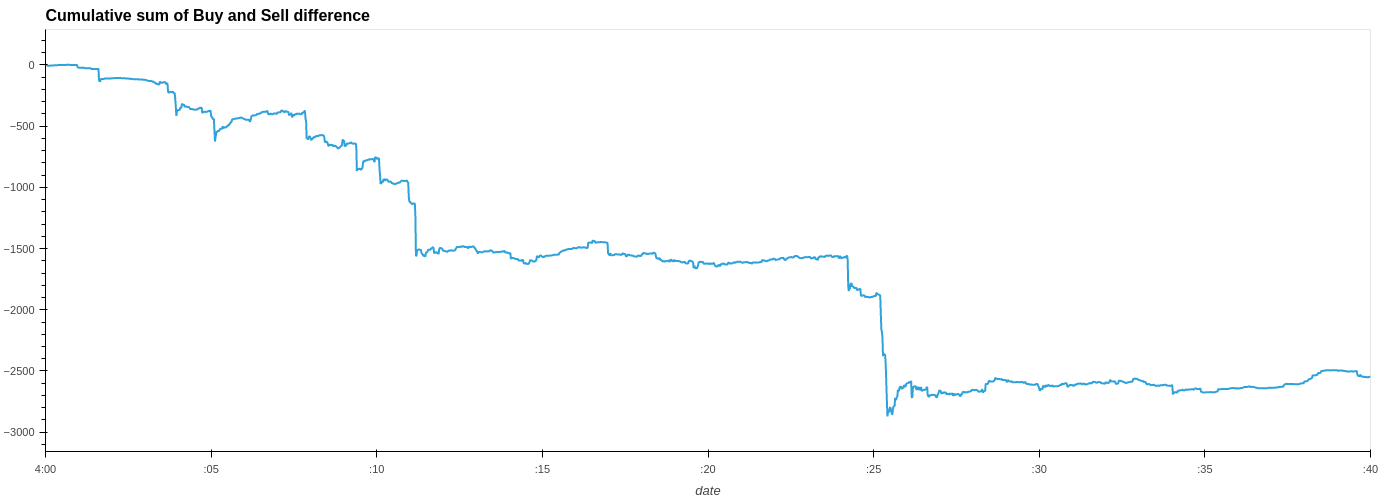
\includegraphics[width=12cm, height = 4cm]{hawkeszoom3.png} \\
    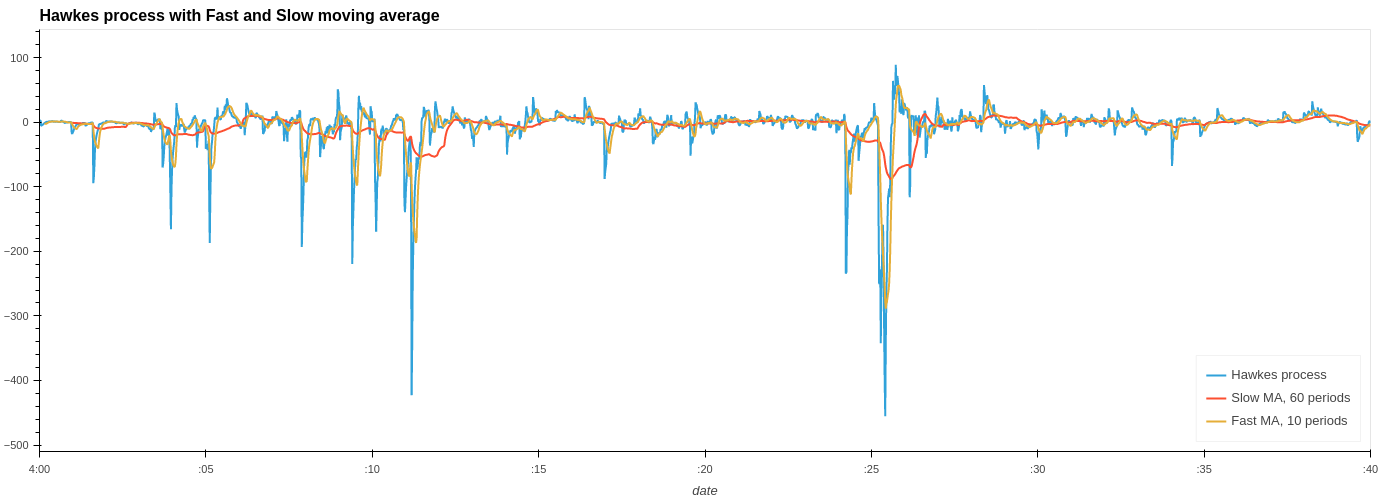
\includegraphics[width=12cm, height = 4cm]{hawkeszoom4.png}
	\caption{Several plots of a 'Hawkes process' on the difference of buy and sell volume along with an example of sampling using moving averages on the above process (in 'seconds' timeframe).}
    \label{fig:hawkeszoom}
\end{figure}


In 2020-10-16 from 04:00 to 04:40, there was a rapid correction in BTCUSD(T) pair. The figure \ref{fig:hawkeszoom}, presents the 'Hawkes process' on the buy and sell volume difference, and then a sampling effort on this process. At first, the third plot (Cumulative sum of Buy and Sell difference), shows that the sell volume is greater than the buy volume. There are also some points where the sell pressure is higher and periods where buy and sell volume are approximately the same. We observe that in the points where imbalance between buy and sell volume occurs, the 'Hawkes process' spikes and then returns at the mean level (which was set at zero). 

The Fast MA (10 periods - orange colour) and Slow MA (60 periods - red colour), cross each other and produce the green circle and red cross of the second plot (Fast MA above or bellow slow MA). The rationale behind this sampling, is that when a falling fast MA crosses a falling slow MA, the price falls (and vice verca), and thus a red arrow of the first plot is accompanied with a red cross of the second plot. Since the 'first point sampled' represents the beginning of one move, the next point that must be sampled, should signify the end of it, where a rising fast MA crosses a falling slow MA. This way, we can sample the beginning (or close to beginning) and the end of the move. Nevertheless, if the price begins to fall gradualy, with no major spikes on the 'Hawkes process', and the fast and slow MA slowly converge, there would be no sampling. Furthermore, this way of sampling is very sensitive to the parameters chosen (fast and slow MA) and as we can see in the second and fourth plot of figure \ref{fig:hawkeszoom}, there are times that the fast is not fast enough to catch the very fast price moves, but does a better job in sampling correctly the larger moves along with their ending.

\subsubsection{Positive and Negative Volume}


From a market microstructure perspective, the search of imbalances of signed volumes (positive volume and negative volume), could reveal the presence of information \cite{marcos}. Based on the work of de Prado, a more precise way of sampling, is to sample when imbalances become apparent in the market. These imbalances could be seen as new information. At this point we need to be precise as to what we will mean from now on, when we the word 'imbalance' is used: deviation of a feature, from our expectation that is calculated from its immediate past (short or long past depending on the parameters chosen). Soon after the imbalance occurs, a new expectation is created that changes as well as new data arrive.

The 'Hawkes process' of the previous subsection, is used in order to sample the imbalances on the difference between buy and sell volume. A very similar way of sampling will be attempted here as well, by changing the 'buy' and 'sell' with 'positive' and 'negative'. We begin by calculating the sign \(b_t\) of returns \(r_t\):
\[ 
b_t =
\begin{cases}
b_{t-1} \text{ for } r_t = 0 \\
\text{sign}(r_t) \text{ for } r_t \neq 0
\end{cases}
\]

The above calculation results to an array with \(\{1,-1\}\), depending on the sign of the returns. Lets denote with \( v_t \) an array that corresponds to the tick by tick volume, and also keep in mind that those arrays get updated as new data arrive. By multiplying the two arrays row by row (hadamard multiplication), the array created, has the same values as \( v_t \) but signed as positive or negative based on the returns. This array will be used in order to sample any imbalances found to the positive or the negative side. One way to do the sampling is the proposed by de Prado way, where 
\[ \theta_T = \max(\sum_{t = t_0}^{T} b_tv_t) \]
represents the imbalance on a non fixed interval of length, \(T\) number of ticks. Then the expectation of the next imbalance \( \mathbb{E}_0(\theta_T) \) is computed using the expectation of the next bars length \( \mathbb{E}_0(T) \) using the next formula:
\[ \mathbb{E}_0(\theta_T) = \mathbb{E}_0(T) \max\{P[b_t=1]\mathbb{E}_0[v_t|b_t=1], (1-P[b_t=1])\mathbb{E}_0[v_t|b_t=-1]\} \]
The above way of sampling is called \textit{Volume Runs Bars} \cite{marcos}.

